%% ****** Start of file aiptemplate.tex ****** %
%%
%%   This file is part of the files in the distribution of AIP substyles for REVTeX4.
%%   Version 4.1 of 9 October 2009.
%%
%
% This is a template for producing documents for use with 
% the REVTEX 4.1 document class and the AIP substyles.
% 
% Copy this file to another name and then work on that file.
% That way, you always have this original template file to use.

%\documentclass[aip,graphicx]{revtex4-1}
%\documentclass[aip,reprint]{revtex4-1}

%\usepackage{graphicx}

%\draft % marks overfull lines with a black rule on the right
\documentclass[pre,aps,floatfix,authordate1-4,twocolumn]{revtex4-1}
%\documentclass[pre,aps,floatfix,authordate1-4]{revtex4-1}

%\documentclass[aps,prl,preprint,superscriptaddress]{revtex4}



%\documentclass[aps,prl,preprint,groupedaddress]{revtex4}

\usepackage{rotating} 
\usepackage{times}
\usepackage{graphicx}
\usepackage{setspace}
\usepackage{amsmath}
\usepackage{epstopdf}
\usepackage[obeyFinal]{easy-todo}
\begin{document}

% Use the \preprint command to place your local institutional report number 
% on the title page in preprint mode.
% Multiple \preprint commands are allowed.
%\preprint{}

\title{Rotational dynamics of proteins from spin relaxation rates and molecular dynamics simulations} %Title of paper

% repeat the \author .. \affiliation  etc. as needed
% \email, \thanks, \homepage, \altaffiliation all apply to the current author.
% Explanatory text should go in the []'s, 
% actual e-mail address or url should go in the {}'s for \email and \homepage.
% Please use the appropriate macro for the type of information

% \affiliation command applies to all authors since the last \affiliation command. 
% The \affiliation command should follow the other information.

\author{O. H. Samuli Ollila}
\email[]{samuli.ollila@helsinki.fi}
%\homepage[]{Your web page}
%\thanks{}
\altaffiliation{Department of Neuroscience and Biomedical Engineering, Aalto University}
\affiliation{Insititute of Biotechnology, University of Helsinki}

% Collaboration name, if desired (requires use of superscriptaddress option in \documentclass). 
% \noaffiliation is required (may also be used with the \author command).
%\collaboration{}
%\noaffiliation

\date{\today}

\begin{abstract}
  % insert abstract here
  
\end{abstract}

%\pacs{}% insert suggested PACS numbers in braces on next line

\maketitle %\maketitle must follow title, authors, abstract and \pacs

% Body of paper goes here. Use proper sectioning commands. 
% References should be done using the \cite, \ref, and \label commands


%\label{}
\section{Introduction}
Protein conformational sampling and entropy
plays significant role in protein functionality
and interactions with other biomolecules.
The related Protein backbone and side chains dynamics 
as well as protein overall brownian tumbling
can be experimentally studied by using NMR relaxation experiments of backbone N-H
or side chain ?? bonds \cite{jarymowycz06,korzhnev01,bedem15}.
Spin relaxation data is usually analyzed by describing the sampled bond
orientations with order parameter $S^2$ respect to the protein reference frame
and assuming that overall and internal motions are independt \cite{??,korzhnev01}.
Order parameters and timescales for overall and internal motions can be then
extracted by fitting various functional forms to spin relaxation data
measured with different magnetic field strengths \cite{jarymowycz06,korzhnev01}.

This approach has been successfully applied for large amount of proteins
with isotropic shape and overall rotational diffusion \cite{jarymowycz06}.
The resulting order parameters and overall rotational diffusion coefficients
have been used in wide range applications, including analysis of conformational
entropy \cite{??}, binding entropy of ?? \cite{??}, resolving sampled structures \cite{??}
and validating molecular dynamics simulations \cite{??}.
%, however, proteins
%with anisotropic shape or large amount of internal motional timescales
%are 
%proteins parameter space for fitted parameters become
%rotational diffusion and internal flexibility of proteins and other biomolecules.
%On the other hand, segmental level information has been used in validation
%and improvement of molecular dynamics simulation force fields \cite{??}.
%Segmental order has been also related to conformational entropy of proteins \cite{??}.

Two different approaches have been commonly used to analyze
rotational dynamics from NMR relaxation experiments. In
''model free analysis'' the fundamental idea is to separate
interal dynamics from global rotation and assume exponential
forms for rotational correlation functions. The parameters of
rotational correlation functions are then fitted the experimental
data to solve time scales and order parameters for different dynamical
processes \cite{??}. Alternative approach is to use bead models and hydrodynamical
calculations to describe protein dynamics and predict spin relaxation rates \cite{??}.
The approaches have been successfull or several proteins, but both suffer
from significant limitations which limit the general applicability \cite{??}.
Main practical issue in the ''model free analysis'' is that the amount of
freen parameters to be fitted in the experiments becomes large for anitoropic
proteins experiencing complex dynamics \cite{??}. On the other hand,
hydrodynamical calculations are sentitive for the assumptions about
protein hydration shell \cite{??}.
 
Classical molecular dynamics simulations have been considered as a
promising tool for interpretation of rotational motions from NMR
relaxation data, because they simultaneously contain internal rotation,
global browian tumbling, anisotropy and hydration shell effects \cite{??}.
However, practical applications have been limited by the inaccuracies
in force field descriptions and available time scales in the simulations.
The most used water model in rotational dynamics studies, tip3p \cite{??},
predicts too fast rotational diffusion \cite{??}. On the other hand, very long
simulations are needed to collect enough statistics to calculate rotational
correlation functions from single molecules in MD simulations \cite{??}.
Consequnetly, protein rotational diffusion coefficients are not typically
calculated from simulation data. Instead, the calculated relaxation rates
are fitted to experiments by assuming an isotropic diffusion model \cite{??}.

In this work we overcome these issues by directly calculating diffusion
coefficients from protein intertia axes. Diffusion coefficients can be then
used to determine global rotational correlation functions from shorter simulations
than with direct calculation. Furthermore, the oversestimated dynamics due to water model
can be anisotropically corrected by scaling the diffusion coefficients with a constant
factor. The usefullness of the approach is demonstrated by interpreting the
spi relaxation data from aniotropic protein constructs from TonB
of Helicobacteri pyroli \cite{??} and Pseudomonas \cite{??}.
These segments are considered as vital parts related to iron transport
into Gran-negative bacteria \cite{??}.


\section{Methods}

\subsection{Spin relaxation and rotational dynamics of molecules}

Practical approaches to analyze molecular dynamics from
NMR relaxation data are usually based on the connection between
second order rotational correlation function $C(t)$ of N-H bond
and experimentally measured spin relaxation rates $R_1$, $R_2$
and $R_{\rm NOE}$ through Redfield equations \cite{abragam,kay89}
\begin{equation}\label{R1}
  \begin{aligned}
  R_{1}= & \frac{d_{\rm{NH}}^2N_{\rm{H}}}{20}\bigg[J(\omega_{\rm{H}}-\omega_{\rm{N}})+3J(\omega_{\rm{N}})+6J(\omega_{\rm{N}}+\omega_{\rm{H}})\bigg] \\
        & +\frac{(\sigma \omega_{\rm{N}})^2}{15}j(\omega_{\rm{N}}),
  \end{aligned}
\end{equation}
\begin{equation}\label{R2}
    \begin{aligned}
  R_{2}= & \frac{1}{2}\frac{d_{\rm{NH}}^2N_{\rm{H}}}{20}\bigg[4J(0)+3j(\omega_{\rm{N}})+J(\omega_{\rm{H}}-\omega_{\rm{N}})+6J(\omega_{\rm{H}})  \\
    & +6J(\omega_{\rm{N}}+\omega_{\rm{H}})\bigg]+\frac{(\sigma \omega_{\rm{N}})^2}{15*6}[4J(0) +3J(\omega_{\rm{N}})],
    \end{aligned}
\end{equation}
\begin{equation}\label{NOE}
R_{\rm NOE}=1+\frac{d_{\rm{NH}}^2N_{\rm{H}}}{20}\bigg[6J(\omega_{\rm{N}}+\omega_{\rm{H}})+J(\omega_{\rm{H}}-\omega_{\rm{N}}))\bigg]\frac{\gamma_{\rm{H}}}{\gamma_{\rm{N}}R_1},
\end{equation}
where $\omega_{\rm{N}}$ and $\omega_{\rm{H}}$ are the Larmor angular
frequencies of $^{15}$N and $^1$H respectively, and
$N_{\rm{H}}$ is the number of bound protons.
Spectral density $J(\omega)$ is the Fourier transformation of the second order
rotational correlation function for N-H bond
\begin{equation}\label{SPECTdens}
  J(\omega)=2\int_0^\infty C(t) \cos(\omega t) {\rm d}t.
\end{equation}
The second order rotational correlation is defined as
\begin{equation}\label{CORRFdef}
  C(t)=\langle (3\cos^2\theta_{t';t'+t}-1)/2 \rangle_{t'},
\end{equation}
where average is ensemble average and $\theta$ is the angle between N-H bonds at times $t'$ and $t'+t$.
The dipolar coupling constant is given by
\begin{equation}
d_{\rm{NH}}=-\frac{\mu_0\hbar\gamma_{\rm{H}}\gamma_{\rm{N}}}{4\pi\langle r_{\rm{CN}}^3\rangle},\nonumber
\end{equation}
where $\mu_0$ is the magnetic constant or vacuum permeability, $\hbar$ is the reduced Planck constant,
$\gamma_{\rm{N}}$ and $\gamma_{\rm{H}}$ are the gyromagnetic constants of $^{15}$N and $^1$H, respectively.
Average cubic length is $\langle r_{\rm{CN}}^3\rangle \approx$ and the 
chemical shift anisotropy is $\Delta \sigma \approx 160*10^{-6}$ for N-H bonds in proteins \cite{??}.
Same equations can be used, for example, to C-H bond by changing the
constants related to nitrogen to the ones corresponding carbon. 

Experimental spin relaxation rates of proteins are typically intepreted by
assuming that the global and interal rotational dynamics are independent.
The rotational correlation function for each bond can be then written as \cite{??}
\begin{equation}\label{CORRFsep}
  C(t)=C_I(t)C_O(t),
\end{equation}
where $C_I(t)$ and $C_O(t)$ are correlation functions for internal and overall
rotiations, respectively. Within this approximation 
the internal rotational correlation function decays to a plateau, which
defines the square of order parameter respect to molecular axes $S^2$.
Timescale for internal relaxation dynamics can be estimated by using the
effective internal correlation time 
\begin{equation}
  \tau_{\rm eff}=\int_0^\infty C_I'(t) \mathrm{d}t,
\end{equation}
where $C_I'(t)=(C_I-S^2)/(1-S^2)$ is the reduced correlation function \cite{??}.

The global rotational dynamics for fully anisotropic molecule
can be described as a sum of five exponentials \cite{??}
\begin{equation}\label{CORRFanisot}
  C_O(t)=\sum_{j=1}^5 A_j e^{-t/\tau_j},
\end{equation}
where time constants $\tau_j$ are related \footnote{
$\tau_1=(4D_{xx}+D_{yy}+D_{zz})^{-1}$,
$\tau_2=(D_{xx}+4D_{yy}+D_{zz})^{-1}$,
$\tau_3=(D_{xx}+D_{yy}+4D_{zz})^{-1}$,
$\tau_4=[6(D+(D^2-L^2)^{-1/2}]^{-1}$,
$\tau_5=[6(D-(D^2-L^2)^{-1/2}]^{-1}$,
$D=\frac{1}{3}(D_{xx}+D_{yy}+D_{zz})$ and 
$L^2=\frac{1}{3}(D_{xx}D_{yy}+D_{xx}D_{zz}+D_{yy}D_{zz})$} to
the diffusion constants around
three principal axes of a molecule
($D_{xx}$, $D_{yy}$ and $D_{zz}$)  and prefactors $A_j$
can be related to the directions of bond respect to the
principal axes.
The rotational diffusion constants are defined as 
\begin{equation}\label{DIFFdef}
  \begin{aligned}
    \langle (\Delta \alpha_{t';t'+t})^2 \rangle_{t'} = 2 D_{xx} t \\
    \langle (\Delta \beta_{t';t'+t})^2 \rangle_{t'} = 2 D_{yy} t \\
    \langle (\Delta \gamma_{t';t'+t})^2 \rangle_{t'} = 2 D_{zz} t, \\
  \end{aligned}
\end{equation}
where $\langle (\Delta \alpha_{t';t'+t})^2 \rangle_{t'}$,
$\langle (\Delta \beta_{t';t'+t})^2 \rangle_{t'}$ and
$\langle (\Delta \gamma_{t';t'+t})^2 \rangle_{t'}$ are mean
square angle deviations of protein intertia axes.
%\begin{equation}
%  C'_I(t)= e^{-t/\tau_c},
%\end{equation}

The internal and overall correlation functions are monoexponential for proteins 
with isotropic overall rotational diffusion and single timescale for internal motion. 
The dynamics of such proteins is described with three parameters in the
original ''model free analysis''; internal rotational relaxation time $\tau_e$,
global rotaional relaxation time $\tau_c$ and the order parameter $S^2$.
The values for these parameters can be then determined by fitting the 
Eqs. \ref{R1}-\ref{CORRFanisot} to experimental spin relaxation data \cite{??}.
However, the amount of exponentials needed to describe correlation functions,
and thus the free parameters, in such fit increases if 
proteins experience anisotropic overall diffusion or several internal timescales.
Thus the ''model free analysis'' becomes less applicable for proteins with significant
anisotropy or more complicated internal dynamics.

%Standard analyses of experimental relaxation data usually assume
%fully or axially isotropic overall rotational motion and single
%decay constant for interal motion. Then the free parameters
%($S^2$, $\tau_j$, $A_j$) are fit against spin relaxation data
%from experiments. This gives most likely very good results for
%isotropic molecules for which the assumption of single internal
%motional timescale is reasonable. However, for molecules with
%significant shape anisotropy or several timescales in internal
%motions the amoount parameters to be fitted becomes large compared
%with the typical amount of experimental points.

\subsection{Rotational dynamics from molecular dynamics simulations}\label{MDanalysis}
Classical molecular dynamics simulation gives a trajectory for each atom in
a system as a function of time. These trajectories can be used to
calculate rotational correlation functions for each bond from Eq. \ref{CORRFdef}.
The rotational correlation functions can be further used to calculate the
spin relaxation times through Eqs. \ref{R1}-\ref{SPECTdens} and the resulting
values can be compared to experimental data in order to assess simulation model
quality \cite{??} and interpret experiments \cite{??}.
However, the comparison is often complicated by
the short simulation times \cite{??} and incorrect overall rotational
diffusion due to water models \cite{??}.

Here we use directly calculated overall rotational diffusion constants
directly from Eq. \ref{DIFFdef} and use those to determine 
the rotational correlation functions for global rotational
dynamics accorfing to Eq. \ref{CORRFanisot}. The rotational diffusion coefficients
are determined by fitting a linear line with one fitting parameter (slope) to
the  mean square angle deviation of intertia axes calculated from
simulations (see results and discussion). In contrast, ten parameters should be
determined in a direct fit of Eq. \ref{CORRFanisot} to the rotational
correlation functions calculated from simulations.
Thus, the determination of correlation functions through overall
rotational diffusion constants is numerically more robust and requires
less simulation data for good statistics. In addition, the incorrect
rotational diffusion due to water model can be corrected by scaling
the rotational diffusion constants with a constant factor before
calculating new correlation functions.

The analysis can be divided in essentially six steps: \\
1) Total rotational correlation functions $C(t)$
for protein N-H bonds are calculated from MD simulation trajectory
by applying Eq.~\ref{CORRFdef}. \\
2) Rotational correlation functions for internal
dynamics $C_I(t)$ are calculated from a trajectory from where the overall
rotation of protein is removed. \\
3) The overall and internal motions are assumed to be independent and overall
rotational correlation function is calculated as $C_O(t)=C(t)/C_I(t)$ according to Eq. \ref{CORRFsep}. \\
4) The protein axes of inertia and their mean square deviations as function of
time are calculated from MD simulation trajectory. \\
5) Rotational diffusion constants $D_x$, $D_y$ and $D_z$ are calculated by fitting a straight line
to mean square angle deviations of inertia axes according to Eq.~\ref{DIFFdef}. \\
6) Timescales in Eq.~\ref{CORRFanisot} are calculated from diffusion constants and
weighting factors $A_j$ are determined by fitting the equation to
rotational correlation functions of overall rotational motion $C_0(t)$ determined in step 3). \\
7) New total rotational correlation functions $C_N(t)$ are determined by multiplying
internal correlation function $C_I(t)$ from step 2) by Eq. \ref{CORRFanisot} with
parameters from step 6). Rotational diffusion constants (and $\tau_i$ values in Eq. \ref{CORRFanisot})
can be also divided by a scaling factor at this point to tune overall
rotational diffusion in rotational dynamics model close to experimental value.



\subsection{Simulation and analysis details}
Simulations were ran using Gromacs 5 \cite{abraham15} And Amber ff99SB- ILDN~\cite{lindorff10}
force field for proteins . The proteins were solvated
to tip3p\cite{jorgensen83}, tip4p \cite{jorgensen83} or OPC4 \cite{izadi14} water models.
NMR structures from \cite{??} and \cite{ciragan16} are used as initial structure for 
PaTonB and HpTonB-92, respectively.
Temperature was coupled to desired value with v-rescale thermistat \cite{bussi07} and pressure was 
isotropically set to 1 bar using Parrinello-Rahman barostat \cite{parrinello81}.
Timestep was 2~fs, Lennart-Jones interactions were cut-off at 1.0~nm,
PME~\cite{darden93,essman95} was used for electrostatics and LINCS was used
to constraint all bond lengths \cite{hess07}. Simulation trajectory and related
files are available at [??].
The simulated systems are listed
in Table \ref{ROTdiffCOEFFS}

The rotation is removed by using fit option in {\it gmx trjconv} and rotational
correlation functions are calculated with {\it gmx rotacf} \cite{gromacsMANUAL}.
Intertia axes of protein are calculated with {\it compute\_inertia\_tensor} from
MDTraj python library~\cite{McGibbon2015MDTraj}.
The spectral density was calculated by first fitting the sum of 471 exponentials
having correlation times from 1 ps and 50 ns with logarithmic spacing to the new
correlation function 
\begin{equation}\label{gprime_fit}
C_N(t)=\sum_{i=1}^{N}\alpha_i e^{-t/\tau_i},
\end{equation}
by using the {\it lsqnonneg} routine in MATLAB \cite{matlab}.
The Fourier transform is then calculated by using analytical function
for the sum of exponentials 
\begin{equation}\label{FTanal}
J(\omega) =  4 \sum_{i=1}^{N}\alpha_i\frac{\tau_i}{1+\omega^2\tau_i^2}.
\end{equation}
Similar approach is used previously for lamellar systems in combination
with solid state NMR experiements \cite{nowacka13,ferreira15}.

\begin{table*}[htb]
\centering
\caption{Simulated systems and rotational diffusion coefficients (rad$^2\cdot 10^7$/s) calculated from simulations.
}\label{ROTdiffCOEFFS}
\begin{tabular}{c c c c c c c c c c c c c c c c}
Protein     & Water model & T (K)  &  $t_{\rm sim}$ (ns)   &  $t_{\rm anal}$ (ns)   & D$_{xx}$ &&D$_{yy}$ &&D$_{zz}$ &&D$_{||}$/D$_+$ & &D$_{av}$& &files \\
\hline
PaTonB      & tip4p       & 298    & 400                 &  390                 & 1.81 $\pm$ 0.01 && 2.06$\pm$ 0.03 && 4.55 $\pm$ 0.03 && 2.35 $\pm$ 0.04 && 2.80 $\pm$ 0.02 && \cite{??} \\
PaTonB      & tip4p       & 310    & 400                 &  390                 &  2.60 $\pm$ 0.02 &&  2.22 $\pm$ 0.05& &  5.0  $\pm$ 0.1  & &  2.07 $\pm$ 0.09& &   3.26 $\pm$  0.07 && \cite{??}\\
PaTonB      & OPC4        & 310    & 1200                &  1190                &  2.01 $\pm$ 0.01 && 2.19 $\pm$ 0.01 && 5.01$\pm$ 0.03 && 2.39 $\pm$ 0.02 && 3.07 $\pm$ 0.01 && \cite{??}  \\
HpTonB-92   & tip3p       & 310    & 570           	 &  370                 & 8.25 $\pm$ 0.05 && 7.67 $\pm$ 0.06 && 15.9 $\pm$ 0.3 && 1.99 $\pm$ 0.06 &&  10.6 $\pm$ 0.2 &&  \cite{??} \\
HpTonB-92   & tip3p       & 303    & 800           	 &  790                 & 6.24 $\pm$ 0.02 && 7.04 $\pm$ 0.03 && 11.9 $\pm$ 0.2 && 1.80 $\pm$ 0.03 && 8.40 $\pm$ 0.07 && \cite{??} \\
HpTonB-92   & tip4p       & 310    & 470           	 &  370                 & 3.6 $\pm$ 0.1 && 3.24 $\pm$ 0.01 && 6.3 $\pm$ 0.3 && 1.8 $\pm$ 0.1 && 4.4 $\pm$ 0.2 && \cite{??} \\
HpTonB-92   & tip4p       & 303    & 400           	 &  200                 & 2.7 $\pm$ 0.1 && 2.71 $\pm$ 0.02 && 5.6 $\pm$ 0.5 && 2.1 $\pm$ 0.2 && 3.7 $\pm$ 0.2 && \cite{??} \\
HpTonB-92   & OPC4        & 310    & 800           	 &  790                 & 2.85 $\pm$ 0.01 && 2.70 $\pm$ 0.01 && 5.56 $\pm$ 0.01 && 2.00 $\pm$ 0.01 && 3.70 $\pm$ 0.01 && \cite{??} \\
\end{tabular}
\end{table*}

\section{Results and discussion}

\subsection{Global rotational dynamics of protein}
Mean square angle deviations of protein intertia axes as a function of time
from PsTonB simulations are shown in Fig. \ref{RMASDplot}.
Diffusion coefficients are calculated from linear fits by taking into
account lag times less than hundredth of the total simulation length,
which is expected to give good statistics for rotation of single molecules
in MD simulations \cite{??}. Linear diffusion fit to mean square angle
displacement seems farily good in Fig.~\ref{RMASDplot}, however,
log-log plot shown in \ref{RMASDplotLOG} reveals some anomalous
diffusion behaviour at time scales below 0.12~ns. Here we use diffusion
coeffiecents to include protein overall motion in spin relaxation
calculations and the effect of small anymaly with short timescales
is beyond the scope of the work. 
\begin{figure}[!h]
  \includegraphics[width=8.5cm]{../Figs/RMASDplot.eps}%
  \caption{The intertia tensor angles as a function of time and mean square angular
    deviations for PsTonB simulation with OPC water model.
    \label{RMASDplot}}%
\end{figure}

The results for diffusion constants
from different simulations shown in Table \ref{ROTdiffCOEFFS}
are in line with previous results from experiments \cite{??} and
simulations \cite{??} for more isotropic proteins. As expected,
rotational diffusion is faster in simulations with higher temperature
or smaller protein. Also the larger diffusion constants for simulations
with tip3p are expected due to the low viscosity of the model \cite{??}.

Inclusion of rotational diffusion coefficients in N-H bond
rotational correlation functions is exemplified in in Fig.~\ref{exampleCORRF}
for residue 331 located in alpha helix of PaTonB protein. 
The same analysis is performed also to other bonds and the resulting
correlation functions are used to calculate spin relaxation rates.
As expected, the N-H bond correlation functions calculated from original MD trajectories
shown in Fig.~\ref{exampleCORRF} A)  decay to fluctuate approximately around zero
after $\sim$20ns. Fluctuations from
ideal relaxation behaviour begin already close to one
hundredth of total simulation time (approximately 4-12ns for the studied systems),
which is expected to be the limit for good
statistic for rotational dynamics analyzed from single molecule MD simulation \cite{??}.
Internal correlation functions, calculated from trajectory with overall protein rotation removed,
in Fig.~\ref{exampleCORRF} B) show rapid decay to a plateau value, which defines the square of the order
parameter $S^2$. The global rotational correlation functions calculated as $C_O(t)=C(t)/C_I(t)$
are shown in Fig.~\ref{exampleCORRF} C). 
\begin{figure}[!h]
  \includegraphics[width=8.5cm]{../Figs/exampleCORRF2.eps}%
  \caption{Example correlation functions for residue 331 of PsTonB calculated from MD simulations with different water models.
    A) total correlation functions $C(t)$ calculated from MD simulation (solid lines) and
    new correlation functions determined from Eqs. \ref{CORRFsep} and \ref{CORRFanisot} by
    using rotational diffusion constants and fitted prefactors (see section \ref{MDanalysis}) (dashed lines),
    B) correlation function for internal motions and %  $S^2$ values determined from the plateau,
    C) correlation function for overall motions determined from Eq. \ref{CORRFsep} ($C_O(t)=C(t)/C_I(t)$) (solid lines) and
    fits to Eq. \ref{CORRFanisot}.
    }\label{exampleCORRF}
\end{figure}

Overall rotational correlation functions were fit to Eq.  \ref{CORRFanisot}, where
timescales for anisotropic rotation~\cite{Note1} were determined by using rotational diffusion constants
from Table \ref{ROTdiffCOEFFS}, to determine the prefactors $A_j$ for all residues.
Resulst for such fit are exemplified with dashed lines in Fig. \ref{exampleCORRF} C) for residue 331 of PsTonB.
The prefactors, global rotational timescales and correlation functions for internal relaxation
were used to determine new correlation function $C_N(t)=C_I(t)\sum_{j=1}^5 A_j e^{-t/\tau_j}$,
where internal correlation comes directly from MD simulation and global rotational correlation
function from diffusion coefficients calculated from MD and Eq. \ref{CORRFanisot}. The new correlation
functions are exemplified with dashed lines in Fig. \ref{exampleCORRF} A) for residue 331 of PsTonB.

%\begin{table}[htb]
%\centering
%\caption{
%}\label{ROTdiffCOEFFSps}
%\begin{tabular}{c c c c c c c}
%                    & &   TIP4P (298K)    & &   TIP4P (310K)       & &          OPC (310K) \\
%D$_{xx}$             & &                   & &  2.60 $\pm$ 0.02     & &         0.020 \\
%D$_{yy}$             & &                   & & 2.22 $\pm$ 0.05      & &  0.022 \\
%D$_{zz}$             & &                   & &  5.0  $\pm$ 0.1      & & 0.048 \\
%D$_{||}$/D$_+$        & &                   & &  2.07 $\pm$ 0.09    & &  2.31 \\
%D$_{av}$            & &                    & &   3.26 $\pm$  0.07   & &     0.030 \\
%tau1     & &     5.67	 & &         6.70 \\
%tau2     & &     6.05	 & &         6.47 \\
%tau3     & &     4.06	 & &         4.29 \\
%tau4      & &    3.45	 & &         3.57 \\
%tau5      & &    9.83	 & &         12.87 \\
  %\hline
%\end{tabular}
%\end{table}

\subsection{Global rotational dynamics in simulations and experiments}
These issues have been typically
overcame by introducing isotropic rotational diffusion term in the correlation
functions \cite{??} or comparing order parameters instead of spin relaxation rates \cite{??}.
These approaches are not, however, useful for anitropic proteins and order
parameter comparison is not direct comparison between simulations and experiments in
the case of freely rotating molecules. 



Spin relaxation rates were calculated from MD simulations by using new correlation
functions, where global rotational dynamics is described by Eq. \ref{CORRFanisot}
with timescales from diffusion constants in Table \ref{ROTdiffCOEFFS} and prefactors
fit to the MD simulation data. The results for PaTonB and HpTonB simulations with different
water models are shown in Figs. \ref{PsTonBrelaxationDATA} and \ref{HsTonBrelaxationDATA},
respectivelty. 
\begin{figure}[!h]
  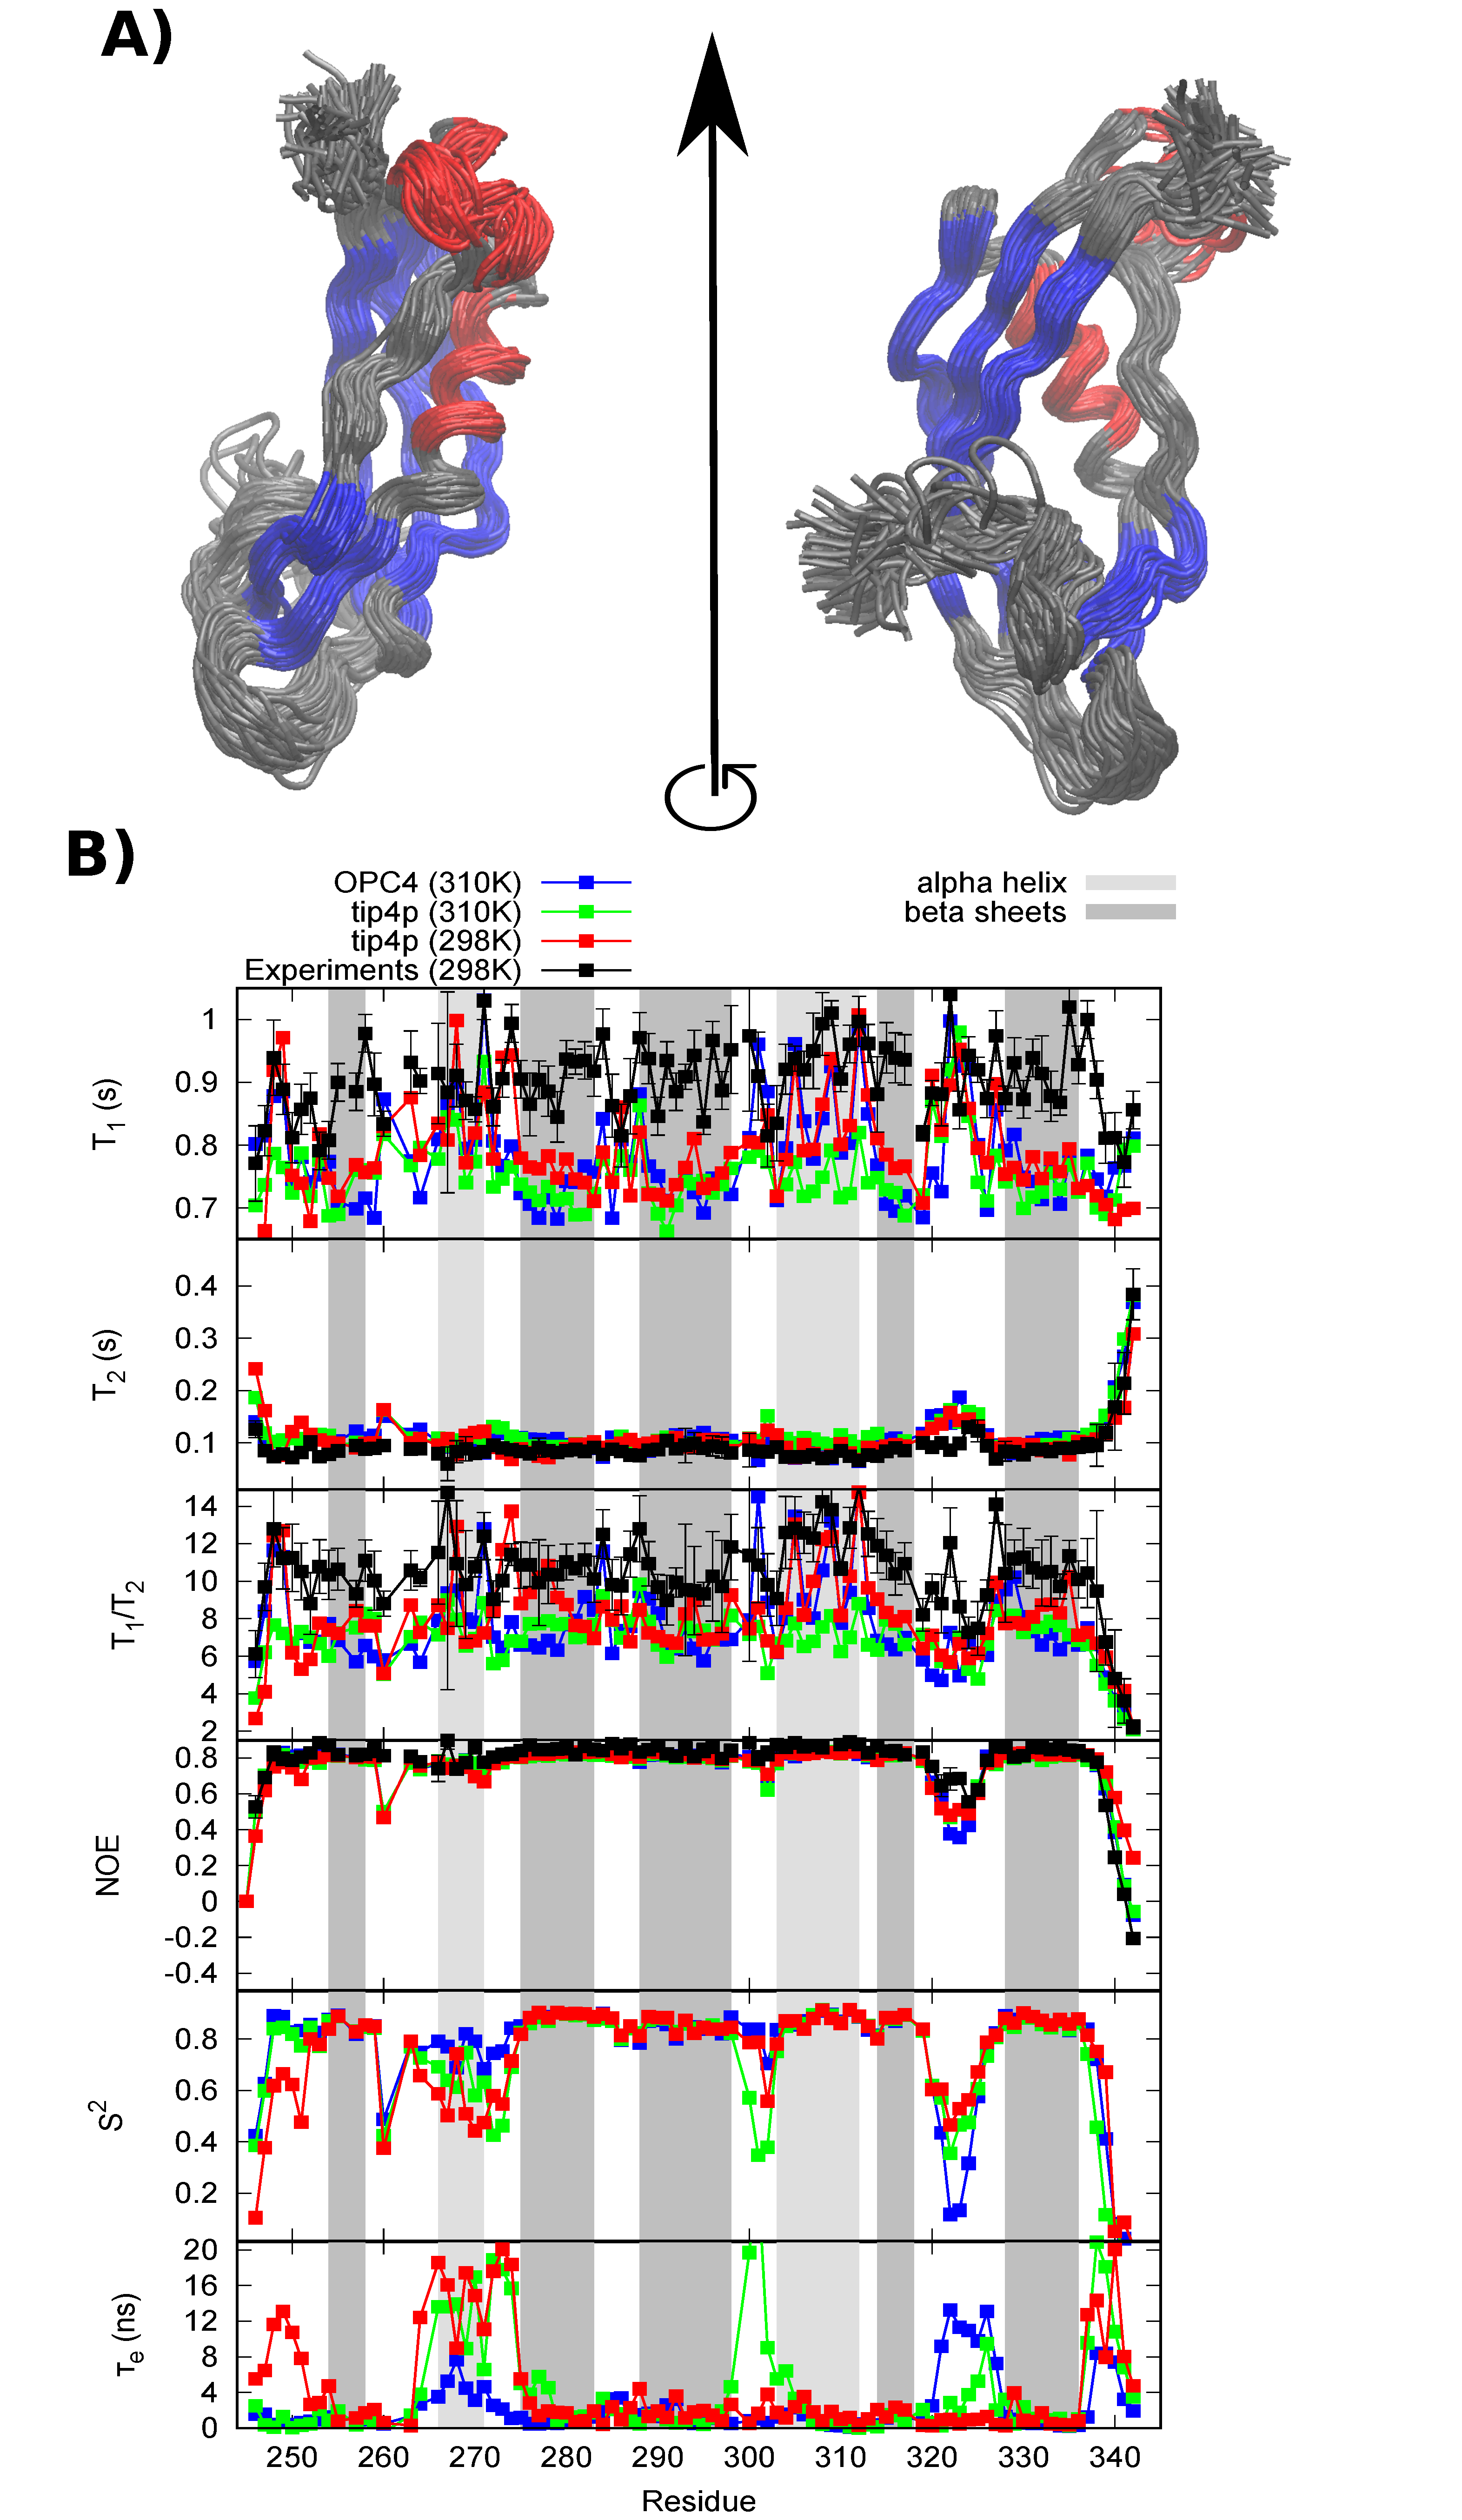
\includegraphics[width=8.5cm]{../Figs/RELdataPsTonB.eps}%
  \caption{A) Structures sampled by PsTonB from MD simulations
    (100 structures from 400ns long trajectory). Alpha helixces are
    shown with red, beta sheets with blue and residues 246-251, 320-326 and 338-342
    with increased internal dynamics are colored yellow.
    Alphahelix sampling between two orientations (residues 266-270) is shown with pink in left column.
    B) Spin relaxation rates, order parameters and effective internal correlation
    times from experiments and simulations.\label{PsTonBrelaxationDATA}}%
\end{figure}
\begin{figure}[!h]
  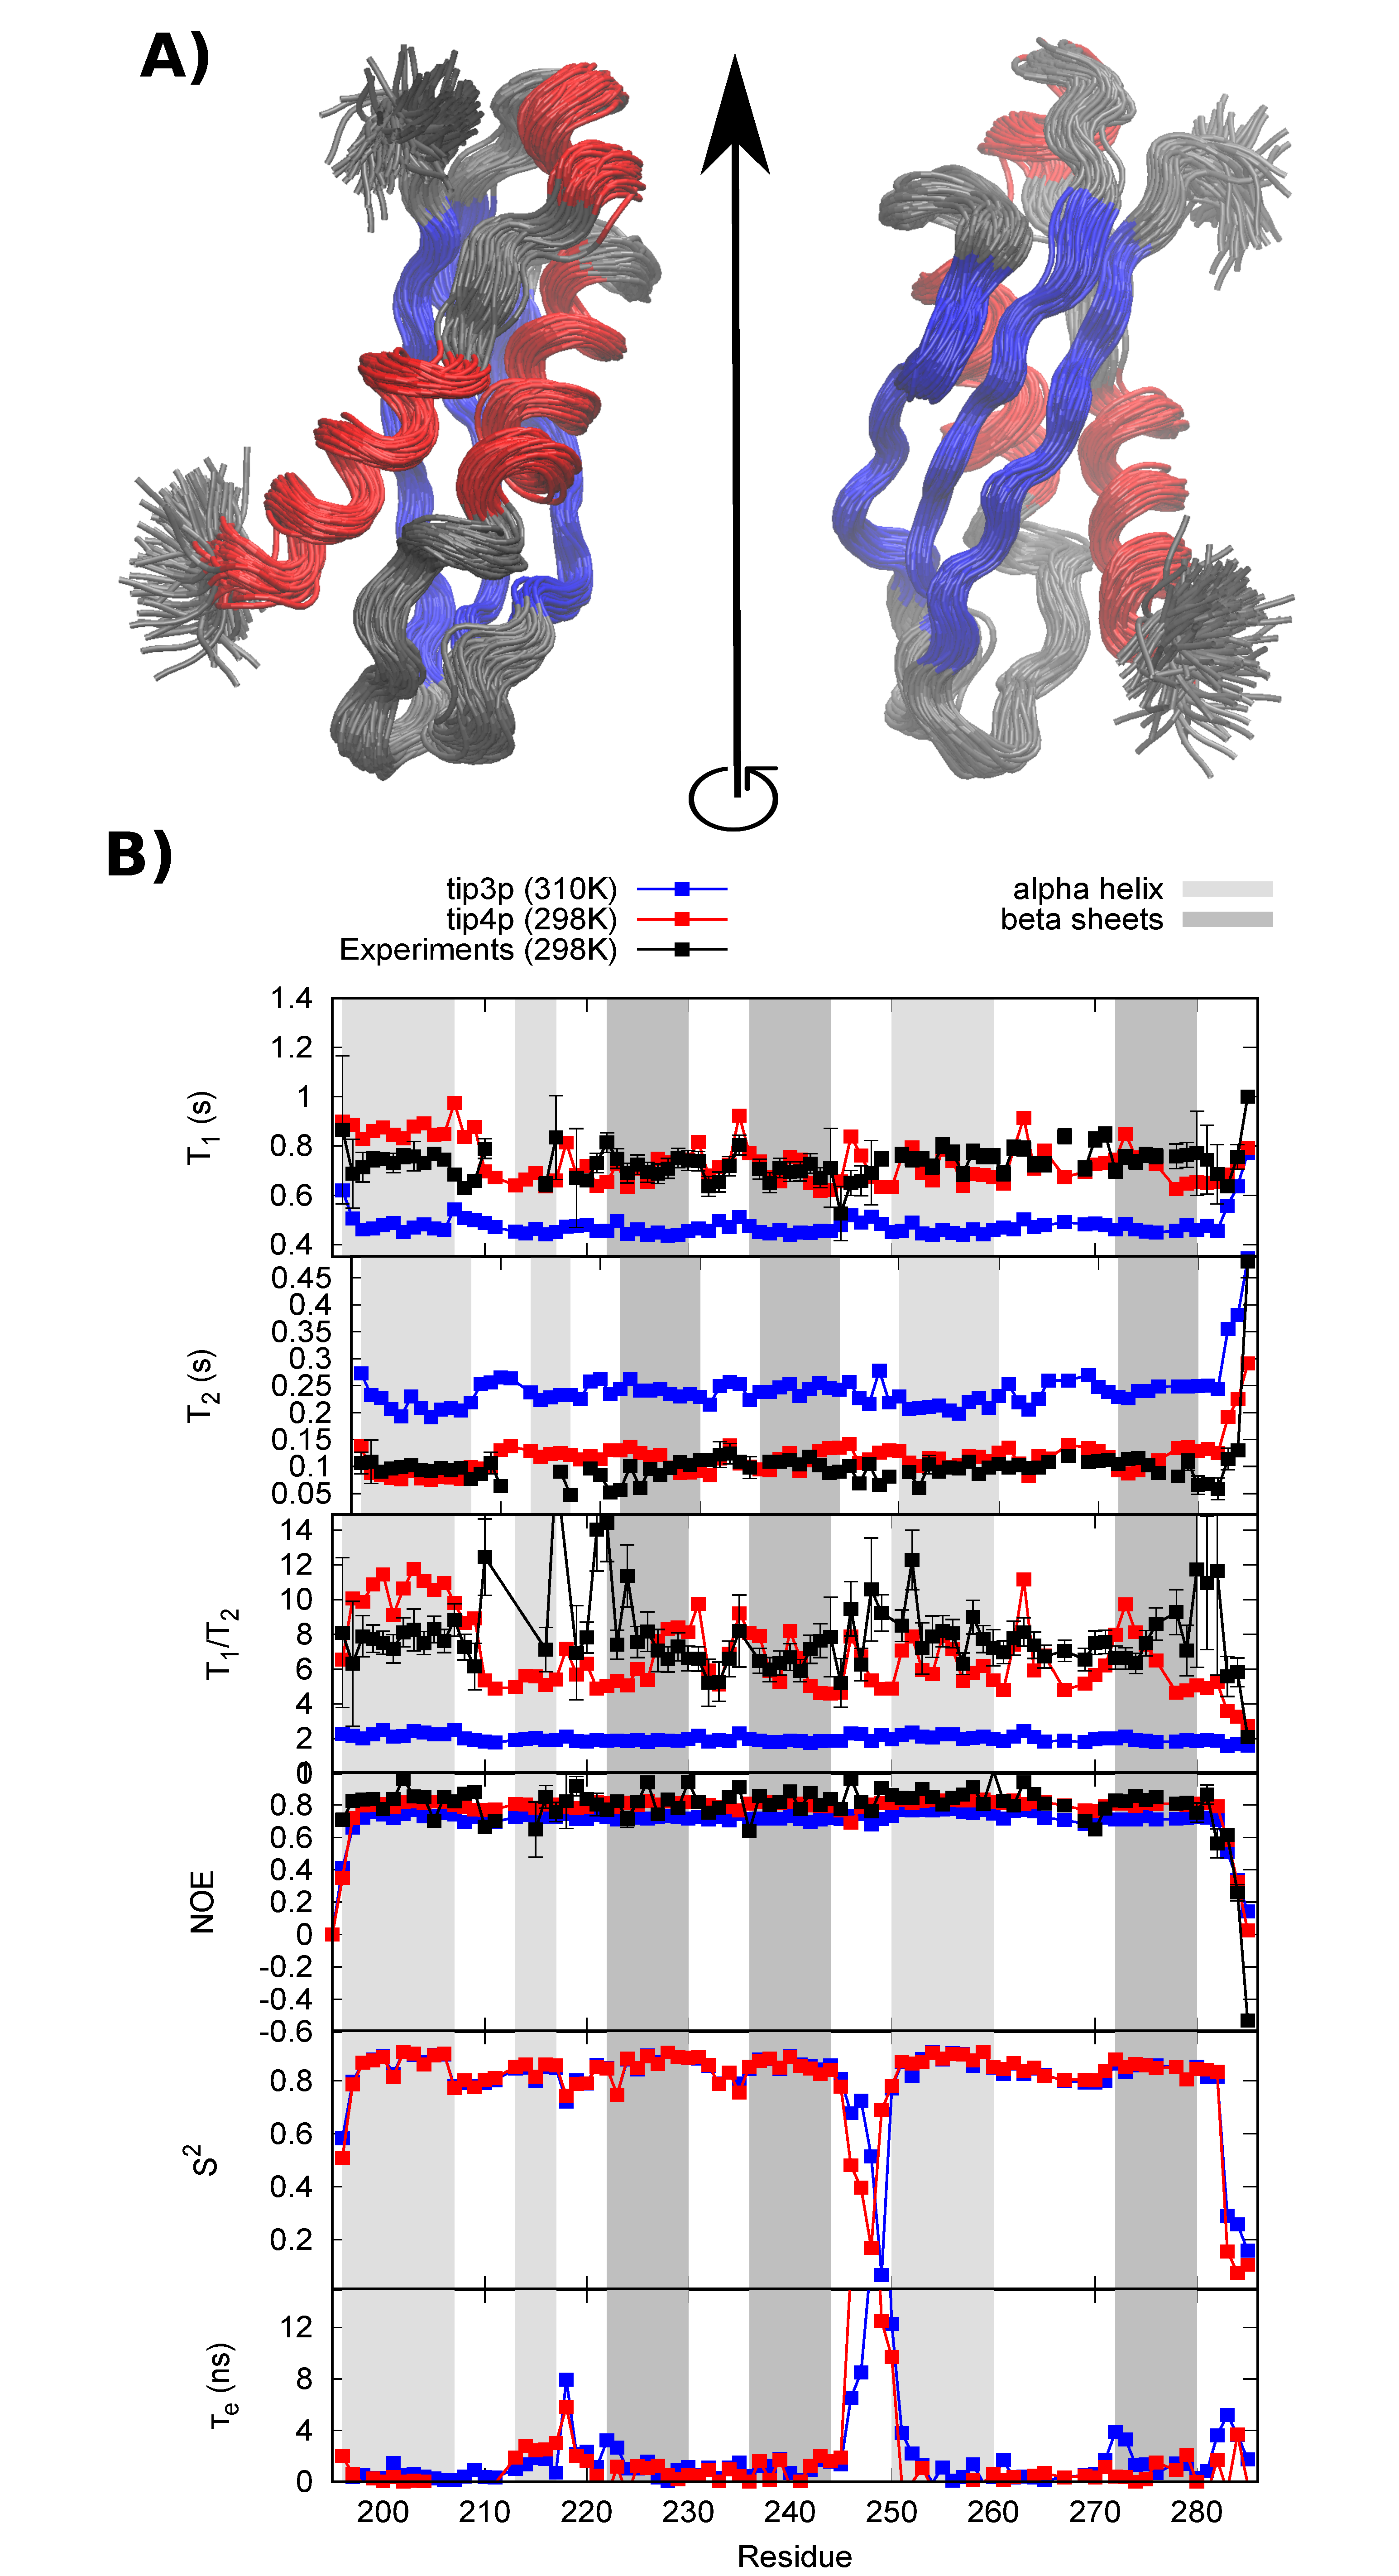
\includegraphics[width=8.5cm]{../Figs/RELdataHpTonB.eps}%
  \caption{Relaxation parameters for HpTonB short construct from
    experiments and simulations with Amber-ildn and different water models
    \label{HpTonBrelaxationDATA}}%
\end{figure}

For PaTonB $T_1$ and $T_1/T_2$ ratio are slightly underestimated  systemically in all simulations.
For HpTonB tip4p gives good agreement with experiments but tip3p results are
significantly off. Underestimation of $T_1/T_2$ ratio suggests that the global rotational
diffusion is overestimated in simulations \cite{??}. Thus, we tested if scaling of
diffusion coefficients with constant factor gives better agreement with experiments. 
%As described in section \ref{MDanalysis}, the global rotational diffusion coefficients
%around all intertia axes can be scaled with a constants and the resulting rotational
%correlation functions can be calculated.
Rotational diffusion coefficients for PaTonB simulation with tip4p and HpTonB simulation with tip3p
were first divided by factors 1.2 and 2.9, respectively. Then, the new correlation functions $C_N(t)$
were calculated by using timescales determined from scaled diffusion constants and prefactors
from the fit to the overall correlation functions. The spin relaxation results from these
correlation functions are shown in Figs. \ref{PsTonBrelaxationDATAscaled} and
\ref{HpTonBrelaxationDATAscaled} for PsTonB and HpTonB, respectively,
are in good agreement with experiments. This suggests that the new correlation functions
with the scaled diffusion coefficients can be used to interpret the protein rotational
dynamics from NMR relaxation data.
\begin{figure}[!h]
  \includegraphics[width=8.5cm]{../Figs/PsTonBrelaxationDATAscaled.eps}%
  \caption{Relaxation parameters for PsTonB from
    experiments and simulations with Amber-ildn and different water models.
    Overall rotational diffusion corrected with factor 1.2.    
    \label{PsTonBrelaxationDATAscaled}}%
\end{figure}
\begin{figure}[!h]
  \includegraphics[width=8.5cm]{../Figs/HpTonBrelaxationDATAscaled.eps}%
  \caption{Relaxation parameters for HpTonB short construct from
    experiments and simulations with Amber-ildn and different water models
    \label{HpTonBrelaxationDATAscaled}}%
\end{figure}


The rotational diffusion coefficients after the scaling are shown in Table \ref{ROTdiffCOEFFSscaled}.
These diffusion constants applied in the global rotational correlation functions give
spin relaxation times in good agreement with experiments, thus these can be considered
as an interperation of NMR relaxation data. The diffusion coefficients from tip3p simulation for HpTonB-92
with scaled diffusion constants (Table \ref{ROTdiffCOEFFSscaled}) and slightly smaller
than diffusion coefficients from tip4p simulation (Table \ref{ROTdiffCOEFFS}), which also
gave a relatively good agreement with experiments. However, the scaled results from
tip3p simulation gives slighltly better agreement for $T_1/T_2$ ratio and, thus, a
better interpretation for experiments.
\begin{table}[!h]
  \centering
  \caption{Rotational diffusion coefficients scaled with constant factor which
    gives a good agreement for spin relaxation data,  2.9 for tip3p simulation of HpTonB
    and by 1.2 for tip4p simulation of PsTonB.}\label{ROTdiffCOEFFSscaled}
  \begin{tabular}{c c c c c}
    &    &  HpTonB-92  &  & PsTonB \\
    \hline
    D$_{xx}$    &   &   2.15 $\pm$ 0.01  & & 1.51  $\pm$ 0.01\\
    D$_{yy}$   &    &  2.43  $\pm$ 0.01  & & 1.72  $\pm$ 0.03\\
    D$_{zz}$   &    &  4.10   $\pm$ 0.01 & & 3.79  $\pm$ 0.03\\
    D$_{av}$  &    &   2.90  $\pm$ 0.03  & & 2.3  $\pm$ 0.02\\
    $\tau_{c}$(ns)  &    &  5.7   $\pm$ 0.1  & & 7.2 $\pm$ 0.1 \\
    %\hline
\end{tabular}
\end{table} 


%\begin{table}[htb]
%\centering
%\caption{Rotational diffusion coefficients (rad$^2\cdot 10^7$/s) calculated from HpTonB-92 simulations}\label{ROTdiffCOEFFShp}
%\begin{tabular}{c c c c c c c }
%            &  &  TIP3P  & &   TIP4P   &  &   OPC \\
%  \hline
%  D$_{xx}$   & &   0.083   & &   0.038   &  &   0.030 \\
%  D$_{yy}$   & &  0.077   &    &   0.033   &  &   0.027 \\
%  D$_{zz}$   & &  0.16    &    &   0.059   &  &    0.058 \\
%  2D$_{zz}$/(D$_{xx}$+D$_{yy}$) &  &   1.99    &  & 1.7    &	&  2.03 \\
%  D$_{av}$  &    &   0.11    &    &   0.043   &  &   0.038 \\
%  tau1     &  &  1.76	 &       &   4.13    &   &   4.87 \\
%  tau2     &  &  1.82	 &       &   4.40    &   &   5.14 \\
%  tau3     &  &  1.26	&        &   3.25    &   &   3.47 \\
%  tau4     &  &  1.05	 &       &    2.75   &   &  2.94 \\
%  tau5     &  &  3.05	 &       &    6.48   &   &   8.43 \\
  
  %\hline
%\end{tabular}
%\end{table} 

%Results with rotational diffusion coefficient corrected with constant factor
%are shown in Fig. \ref{relaxationDATAplotSCALED}. 
%\begin{figure}[!h]
%  \includegraphics[width=13cm]{/Users/osollila/Dropbox/TonB/Figs/relaxationDATAplotSCALED.eps}%
%  \includegraphics[width=13cm]{/home/samuli/Dropbox/TonB/Figs/relaxationDATAplotSCALED.eps}%
%  \caption{Relaxation parameters for HpTonB short construct from
%    experiments and simulations with Amber-ildn and different water models.
%    The rotational diffusion coefficients are divided by 3.0 for tip3p simulation
%    and by 1.3 for tip4p simulation.
%    Experiments are done in 303K and simulations in 310K, simulations in 303K are running.
%    \label{relaxationDATAplotSCALED}}%
%\end{figure}

%\begin{figure}[!h]
%  \includegraphics[width=13cm]{/Users/osollila/Dropbox/TonB/Figs/relaxationDATAplotLONGERconstructSCALED.eps}%
%  \includegraphics[width=13cm]{/home/samuli/Dropbox/TonB/Figs/relaxationDATAplotLONGERconstructSCALED.eps}%
%  \caption{PRELIMINARY RESULTS for relaxation parameters for HpTonB longer construct (107) from
%    experiments and simulations with Amber-ildn and tip4p water models.
%    The rotational diffusion coefficients are divided by 1.3.
%    Experiments and simulations are done in 303K.
%    \label{relaxationDATAplotSCALEDlongerCONSTRUCT}}%
%\end{figure}


%\begin{table}[htb]
%\centering
%\caption{Rotational diffusion coefficients scaled with constant factor which
%  gives a good agreement for spin relaxation data,  3.0 for tip3p simulation
%    and by 1.3 for tip4p simulation.
%  OPC RESULTS TO BE CHECKED.
%}\label{ROTdiffCOEFFS}
%\begin{tabular}{c c c c c c c }
%  rad$^2$/ns   &    &  TIP3P  &   &   TIP4P \\%  &  &   OPC \\
%  \hline
%  D$_{xx}$    &   &   0.028   &   &   0.029 \\%  &  &   0.030 \\
%  D$_{yy}$   &    &  0.026   &    &   0.025 \\%  &  &   0.027 \\
%  D$_{zz}$   &    &  0.053    &    &   0.045 \\%   &  &    0.058 \\
%  2D$_{zz}$/(D$_{xx}$+D$_{yy}$) &  &   1.99    &  & 1.7 \\%   &	&  2.03 \\
%  D$_{av}$  &    &   0.034    &    &   0.033 \\%  &  &   0.038 \\
  %\hline
%\end{tabular}
%\end{table} 



\subsection{Interpretation of protein internal relaxation from MD simulations}
Spin relaxation rates from tip4p simulations for PsTonB are in good agreement with
experimetns (see Figs \ref{??}), thus the simulations can be used to give interpretation
for rotational relaxation processes in proteins, which correspond the
NMR relaxation results. Spin relaxation rate deviations from baseline
are observed for residues 246-251 in N-terminus, residues 320-326
and residues 338-342 in C-terminus. These segments are coloured in yellow
in Fig. \ref{??} A), which already revels ecnhanged conformational sampling
in these regions. Also order parameters are low and effective internal
relaxation times long for these segements as seen in Fig. \ref{??} B).

More detailed interpretation of different relaxation processes experienced
by different residues can be done by analysing timescales which leads in simulation
model to the spin relaxation rates in agreement with experiments. Prefactors
from Eq. \ref{??} fitted in rotational correlation functions in agreement
with spin relaxation data are shown in Fig \ref{coeffsPLOT} for different residues
in PsTonB. Residue 331 represents the last alpha helix before C terminus and its rotational
relaxation is mostly dominated by relaxations with timescales $\sim$5.5~ns and $\sim$8~ns,
which arise from global rotation of protein an only small fraction of relaxation arises from
fast internal motions, in accordance with large order parameter value (??).
Relaxation of residue 322 is also dominated by relaxation processes with timescale
around $\sim$8~ns, but fast motions related to internal protein dynamics are more
significant than for alpha helix residue 331. This explains the low order parameter (??)
measured small NOE and large $T_2$ relaxation times values shown in Fig. \ref{??}.
Rotational dynamics of residue 341 located in N terminus is dominated by the fast
motions related to the internal protein relaxation, as expected from the low order
parameter. The contribution from timescales close to $\sim$13~ns are probably related
to slower conformational sampling of the N terminus, which is also seen in sampled
conformations and large effective correlation times in Fig. \ref{??}.
\begin{figure}[!h]
  \includegraphics[width=8.5cm]{../Figs/coeffsPLOT.eps}%
  \caption{Prefactors $A_i$ corresponding different timescales $\tau_i$ in Eq.\ref{??}
    resulting from a fit in correlation functions giving good agreement with spin
    relaxation rates in experimetns for PsTonB. 
    \label{coeffsPLOT}}%
\end{figure}

In addition, low order parameters and larger effective correlation times
are observed for PsTonB residues 260-274 and 300-303
in Fig. \ref{PsTonBrelaxationDATA} B).
For residues 260-274 this can be explained by two different orientations
sampled by alpha helix on that region, as highlighted with pink
in Fig.~\ref{PsTonBrelaxationDATA} A). This explains also the
lower resolution in NMR spectra observed for this and similar region in
HpTonB structures \cite{??}. Low order parameters and large
effective correlation times between residues 300-303 are not seen
in spin relaxation data, thus it is not clear if these arise from
simulation artefact.

Spin relaxation rate deviations from baseline are observed only few residues in
terminal ends for HpTonB-92 as seen in Fig. \ref{HPTonBrelaxationDATA}.
This is the case also in simulations, except that
the N terminus flexibility seems to be somewhat overestimated and 
low order parameters and long effetive correlation times are also observed
for residues 245-250. The latter observation probably arises
(at least partly) from simulation artefacts because deviation form experimental
relaxation data is relatively large for these residues.
More detailed discussion together with longer HpTonB construct is
presented elsewhere \cite{??}.
%Different orientations of alpha helix between residues 210-220 and
%decreased order parameters are not observed in contrast to PsTonB,
%except single large effective correlation time value at residue 218.
%The low resolution in NMR spectra \cite{??}, however, suggest that
%the same phenomena is present but not observed in simulations, possibly
%due to timescale or force field issues.

\section{Conclusions}

Rotation of protein intertia axes is observed to experience linear
diffusion behaviour and overall diffusion component of rotational 
correlation functions of individual N-H bonds can can be successfully 
fitted to the model assuming anitropic diffusion for whole molecule.

Rotational diffusion of whole molecules is overestimated by a factor
of $\sim$3 in simulations with tip3p water, in agreement with previous
studies \cite{??}. The simulations with tip4p and opc4 water models
give more realistic diffusion coefficients, which overestimate diffusion
only with factors $\sim$1-1.2. 

The overstimated overall diffusion
coefficient can be corrected post-simulationally to compare internal dynamics
and order with experiments. 

The presented methodology can be used to interpret spin relaxation experiments
by using MD simulations \cite{??} and asses the quality of protein force fields
against NMR experiments. The presented scaling of overall anisotropic diffusion
allows this also for simulations with incorrect rotational diffusion due to water
models, which is the case in simulations with tip3p. 

% If you have acknowledgments, this puts in the proper section head.
\begin{acknowledgments}
% Put your acknowledgments here.
%OHSO acknowledges Aalto science IT project and CSC-IT center for science for
%computational resources, and Emil Aaltonen foundation for funding.
\end{acknowledgments}

% Create the reference section using BibTe
\bibliography{refs.bib}

%\newpage
%\appendix
\begin{center}
{\bf SUPPLEMENTARY INFORMATION}
\end{center}
\begin{figure}[!h]
  \includegraphics[width=8.5cm]{../Figs/RMASDplotLOG.eps}%
  \caption{The intertia tensor angles as a function of time and mean square angular
    deviations for PsTonB simulation with OPC water model.
    \label{RMASDplotLOG}}%
\end{figure}

%\todolist
\end{document}
%
% ****** End of file aiptemplate.tex ******
